\section{Simulazioni modello di Ising1D}

%-----------------------------------------%
%				Prima slide				  %
%	   Caratterizzazione del modello   	  %
%-----------------------------------------%
\begin{frame}
    \frametitle{Caratterizzazione}
    \framesubtitle{}

    \begin{columns}
        \begin{column}{0.33\textwidth}
            \begin{block}{Termalizzazione}

                \begin{itemize}[itemsep=0.5em, label=$\diamond$]
                    \item Maggiore T, minore $t_{term}$
                    \item $t_{term}^{max}\,\simeq\,600$ sweeps
                \end{itemize}

                \vspace{0.5cm}

                \centering
                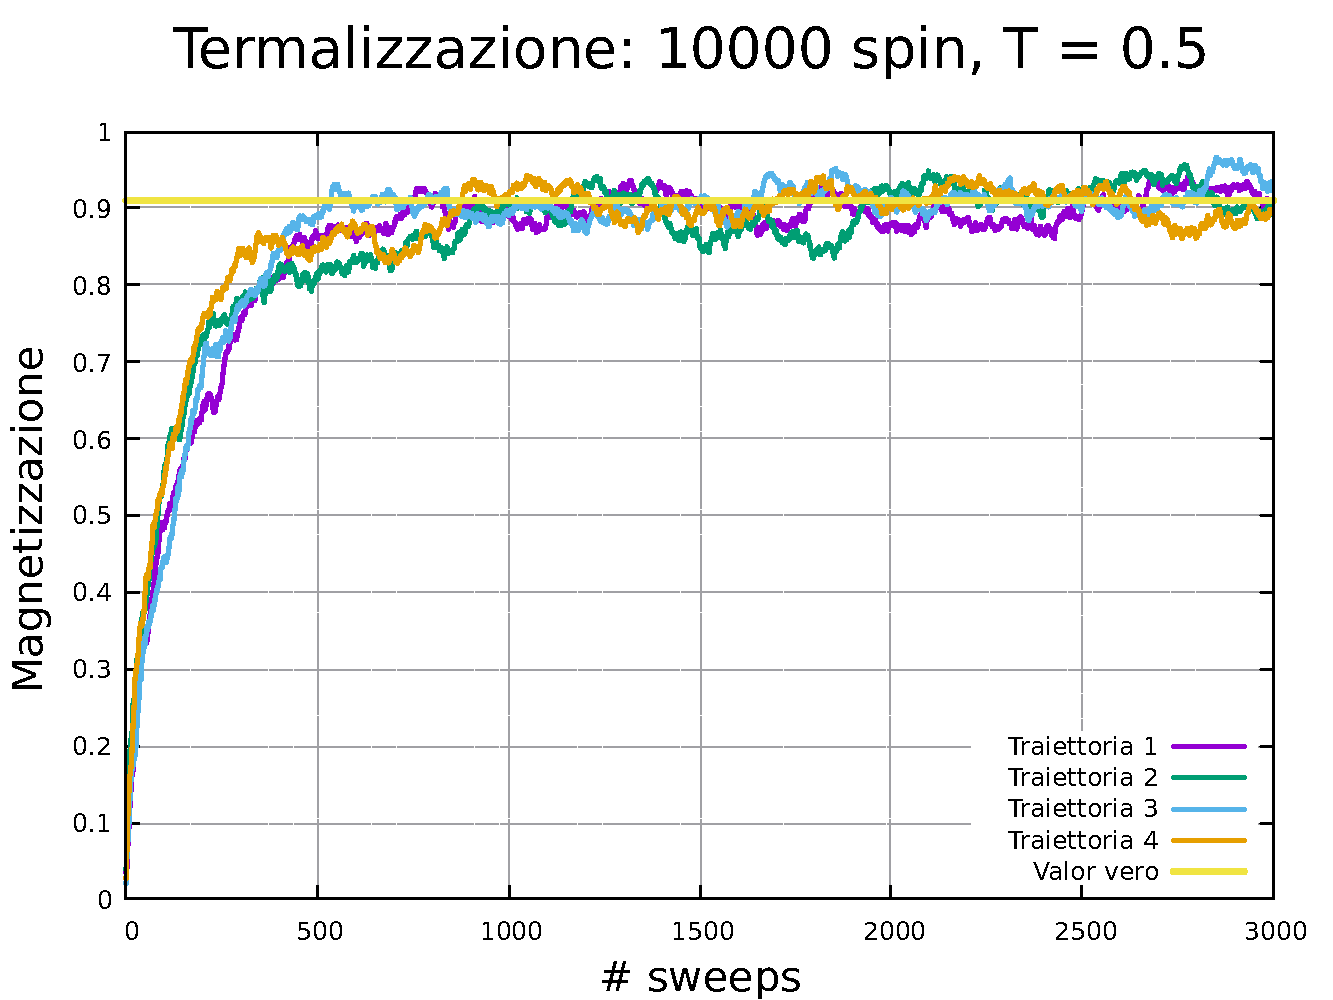
\includegraphics[width=\textwidth]{Immagini/simIsing1D/term_10000_1.5.pdf}
            
            \end{block}
        \end{column}
    
        \begin{column}{0.33\textwidth}
            \begin{block}{Auto-correlazione}

                \begin{itemize}[itemsep=0.5em, label=$\diamond$]
                    \item Maggiore T, minore $t_{c}$
                    \item $t_{c}^{max}\,\simeq\,500$ sweeps
                \end{itemize}

                \vspace{0.5cm}

                \centering
                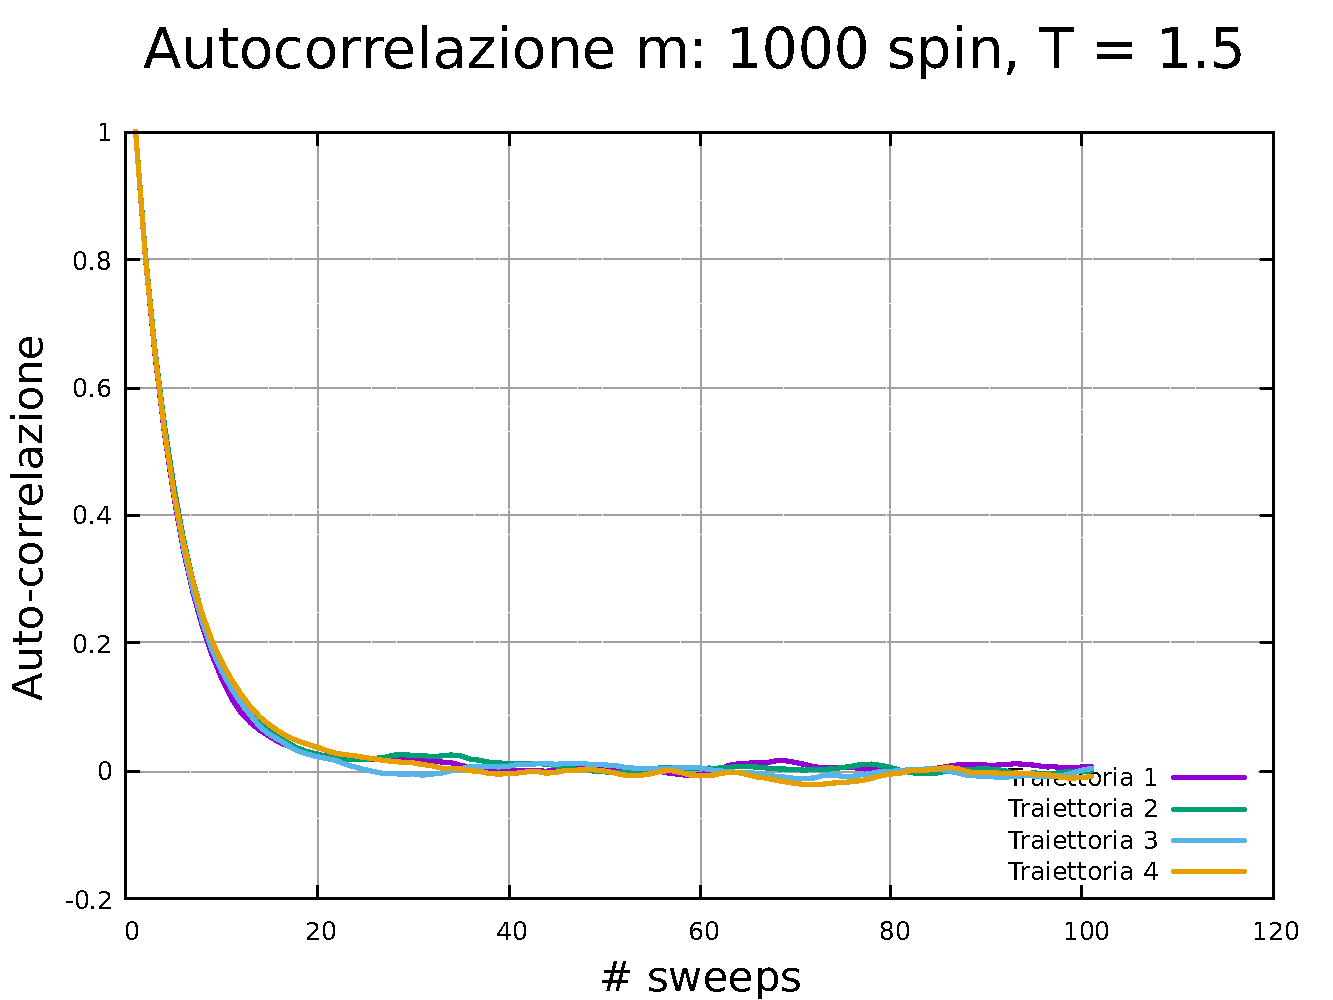
\includegraphics[width=\textwidth]{Immagini/simIsing1D/auto_1000_1.5.pdf}
            
            \end{block}
        \end{column}

        \begin{column}{0.33\textwidth}
            \begin{block}{Blocchi}
                \begin{itemize}[itemsep=0.5em, label=$\diamond$]
                    \item Maggiore T, minore $l_{blk}$
                    \item $l_{blk}^{max}\,\simeq\,1000$ sweeps
                \end{itemize}

                \vspace{0.5cm}

                \centering
                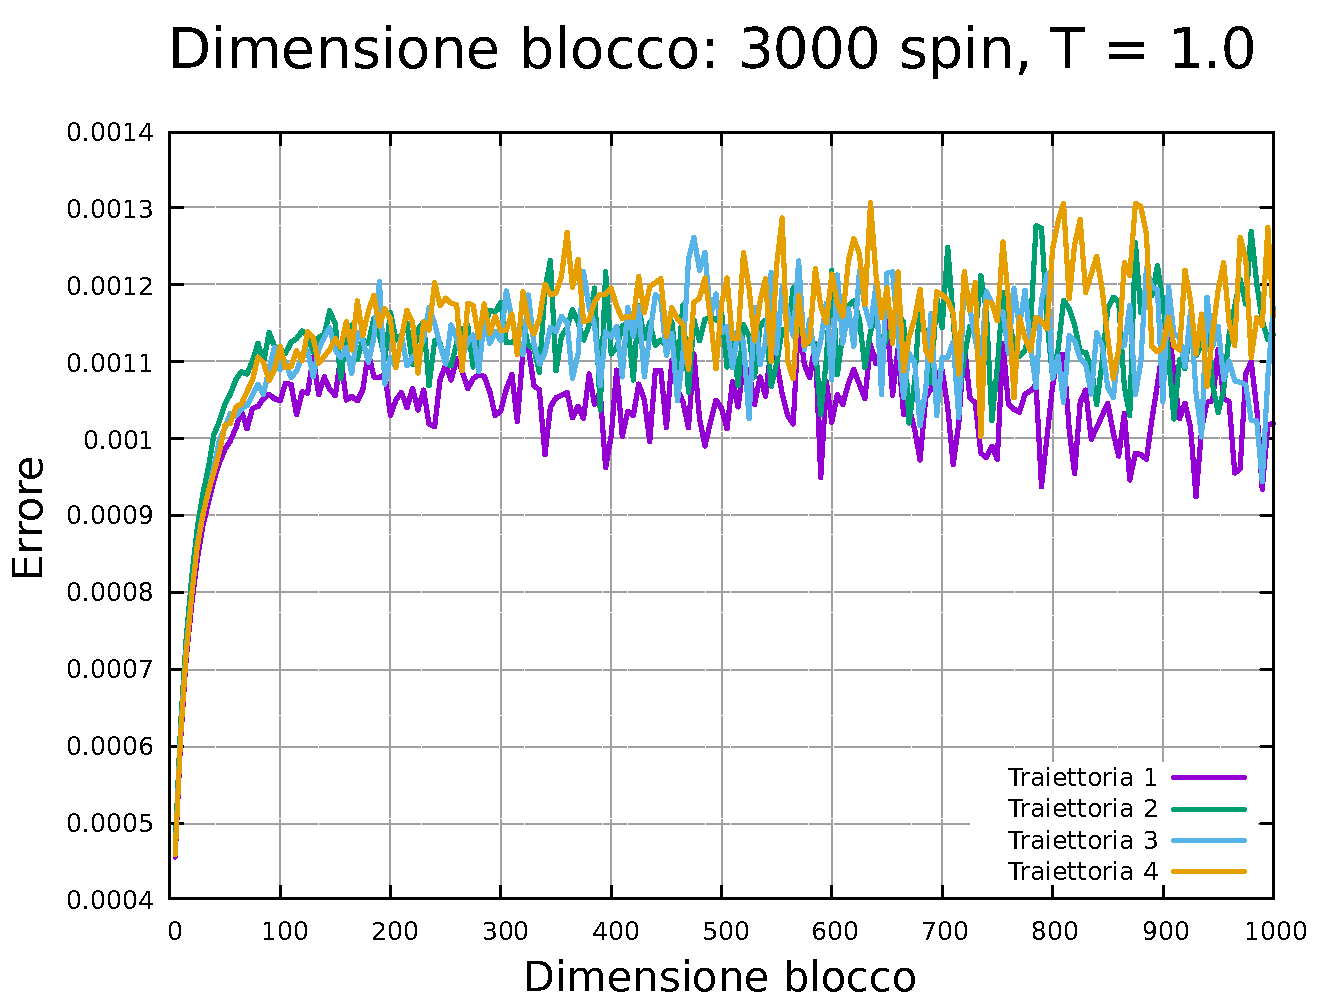
\includegraphics[width=\textwidth]{Immagini/simIsing1D/err_3000_1.0.pdf}
            \end{block}        
        \end{column}
    \end{columns}
\end{frame}